\documentclass[twoside]{book}

% Packages required by doxygen
\usepackage{fixltx2e}
\usepackage{calc}
\usepackage{doxygen}
\usepackage[export]{adjustbox} % also loads graphicx
\usepackage{graphicx}
\usepackage[utf8]{inputenc}
\usepackage{makeidx}
\usepackage{multicol}
\usepackage{multirow}
\PassOptionsToPackage{warn}{textcomp}
\usepackage{textcomp}
\usepackage[nointegrals]{wasysym}
\usepackage[table]{xcolor}

% Font selection
\usepackage[T1]{fontenc}
\usepackage[scaled=.90]{helvet}
\usepackage{courier}
\usepackage{amssymb}
\usepackage{sectsty}
\renewcommand{\familydefault}{\sfdefault}
\allsectionsfont{%
  \fontseries{bc}\selectfont%
  \color{darkgray}%
}
\renewcommand{\DoxyLabelFont}{%
  \fontseries{bc}\selectfont%
  \color{darkgray}%
}
\newcommand{\+}{\discretionary{\mbox{\scriptsize$\hookleftarrow$}}{}{}}

% Page & text layout
\usepackage{geometry}
\geometry{%
  a4paper,%
  top=2.5cm,%
  bottom=2.5cm,%
  left=2.5cm,%
  right=2.5cm%
}
\tolerance=750
\hfuzz=15pt
\hbadness=750
\setlength{\emergencystretch}{15pt}
\setlength{\parindent}{0cm}
\setlength{\parskip}{3ex plus 2ex minus 2ex}
\makeatletter
\renewcommand{\paragraph}{%
  \@startsection{paragraph}{4}{0ex}{-1.0ex}{1.0ex}{%
    \normalfont\normalsize\bfseries\SS@parafont%
  }%
}
\renewcommand{\subparagraph}{%
  \@startsection{subparagraph}{5}{0ex}{-1.0ex}{1.0ex}{%
    \normalfont\normalsize\bfseries\SS@subparafont%
  }%
}
\makeatother

% Headers & footers
\usepackage{fancyhdr}
\pagestyle{fancyplain}
\fancyhead[LE]{\fancyplain{}{\bfseries\thepage}}
\fancyhead[CE]{\fancyplain{}{}}
\fancyhead[RE]{\fancyplain{}{\bfseries\leftmark}}
\fancyhead[LO]{\fancyplain{}{\bfseries\rightmark}}
\fancyhead[CO]{\fancyplain{}{}}
\fancyhead[RO]{\fancyplain{}{\bfseries\thepage}}
\fancyfoot[LE]{\fancyplain{}{}}
\fancyfoot[CE]{\fancyplain{}{}}
\fancyfoot[RE]{\fancyplain{}{\bfseries\scriptsize Generated by Doxygen }}
\fancyfoot[LO]{\fancyplain{}{\bfseries\scriptsize Generated by Doxygen }}
\fancyfoot[CO]{\fancyplain{}{}}
\fancyfoot[RO]{\fancyplain{}{}}
\renewcommand{\footrulewidth}{0.4pt}
\renewcommand{\chaptermark}[1]{%
  \markboth{#1}{}%
}
\renewcommand{\sectionmark}[1]{%
  \markright{\thesection\ #1}%
}

% Indices & bibliography
\usepackage{natbib}
\usepackage[titles]{tocloft}
\setcounter{tocdepth}{3}
\setcounter{secnumdepth}{5}
\makeindex

% Hyperlinks (required, but should be loaded last)
\usepackage{ifpdf}
\ifpdf
  \usepackage[pdftex,pagebackref=true]{hyperref}
\else
  \usepackage[ps2pdf,pagebackref=true]{hyperref}
\fi
\hypersetup{%
  colorlinks=true,%
  linkcolor=blue,%
  citecolor=blue,%
  unicode%
}

% Custom commands
\newcommand{\clearemptydoublepage}{%
  \newpage{\pagestyle{empty}\cleardoublepage}%
}

\usepackage{caption}
\captionsetup{labelsep=space,justification=centering,font={bf},singlelinecheck=off,skip=4pt,position=top}

%===== C O N T E N T S =====

\begin{document}

% Titlepage & ToC
\hypersetup{pageanchor=false,
             bookmarksnumbered=true,
             pdfencoding=unicode
            }
\pagenumbering{roman}
\begin{titlepage}
\vspace*{7cm}
\begin{center}%
{\Large My Project }\\
\vspace*{1cm}
{\large Generated by Doxygen 1.8.11}\\
\end{center}
\end{titlepage}
\clearemptydoublepage
\tableofcontents
\clearemptydoublepage
\pagenumbering{arabic}
\hypersetup{pageanchor=true}

%--- Begin generated contents ---
\chapter{Class Index}
\section{Class List}
Here are the classes, structs, unions and interfaces with brief descriptions\+:\begin{DoxyCompactList}
\item\contentsline{section}{\hyperlink{structnode}{node} }{\pageref{structnode}}{}
\item\contentsline{section}{\hyperlink{structnode1}{node1} }{\pageref{structnode1}}{}
\item\contentsline{section}{\hyperlink{structnode__info}{node\+\_\+info} }{\pageref{structnode__info}}{}
\end{DoxyCompactList}

\chapter{File Index}
\section{File List}
Here is a list of all files with brief descriptions\+:\begin{DoxyCompactList}
\item\contentsline{section}{\hyperlink{Lab1_8c}{Lab1.\+c} }{\pageref{Lab1_8c}}{}
\end{DoxyCompactList}

\chapter{Class Documentation}
\hypertarget{structgrafo}{}\section{grafo Struct Reference}
\label{structgrafo}\index{grafo@{grafo}}


Collaboration diagram for grafo\+:
\nopagebreak
\begin{figure}[H]
\begin{center}
\leavevmode
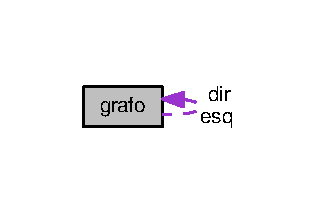
\includegraphics[width=152pt]{structgrafo__coll__graph}
\end{center}
\end{figure}
\subsection*{Public Attributes}
\begin{DoxyCompactItemize}
\item 
struct \hyperlink{structgrafo}{grafo} $\ast$ \hyperlink{structgrafo_a258a14d55dea22c0507102319671226f}{esq}
\item 
struct \hyperlink{structgrafo}{grafo} $\ast$ \hyperlink{structgrafo_acefee7ad605f204f8b1bd063adfac34c}{dir}
\item 
int \hyperlink{structgrafo_a9f3a642f8e0a5350f2a4896d3db685ee}{i}
\end{DoxyCompactItemize}


\subsection{Member Data Documentation}
\index{grafo@{grafo}!dir@{dir}}
\index{dir@{dir}!grafo@{grafo}}
\subsubsection[{\texorpdfstring{dir}{dir}}]{\setlength{\rightskip}{0pt plus 5cm}struct {\bf grafo}$\ast$ grafo\+::dir}\hypertarget{structgrafo_acefee7ad605f204f8b1bd063adfac34c}{}\label{structgrafo_acefee7ad605f204f8b1bd063adfac34c}
\index{grafo@{grafo}!esq@{esq}}
\index{esq@{esq}!grafo@{grafo}}
\subsubsection[{\texorpdfstring{esq}{esq}}]{\setlength{\rightskip}{0pt plus 5cm}struct {\bf grafo}$\ast$ grafo\+::esq}\hypertarget{structgrafo_a258a14d55dea22c0507102319671226f}{}\label{structgrafo_a258a14d55dea22c0507102319671226f}
\index{grafo@{grafo}!i@{i}}
\index{i@{i}!grafo@{grafo}}
\subsubsection[{\texorpdfstring{i}{i}}]{\setlength{\rightskip}{0pt plus 5cm}int grafo\+::i}\hypertarget{structgrafo_a9f3a642f8e0a5350f2a4896d3db685ee}{}\label{structgrafo_a9f3a642f8e0a5350f2a4896d3db685ee}


The documentation for this struct was generated from the following file\+:\begin{DoxyCompactItemize}
\item 
\hyperlink{BinaryTree_8c}{Binary\+Tree.\+c}\end{DoxyCompactItemize}

\chapter{File Documentation}
\hypertarget{BinaryTree_8c}{}\section{Binary\+Tree.\+c File Reference}
\label{BinaryTree_8c}\index{Binary\+Tree.\+c@{Binary\+Tree.\+c}}
{\ttfamily \#include $<$stdio.\+h$>$}\\*
{\ttfamily \#include $<$stdlib.\+h$>$}\\*
Include dependency graph for Binary\+Tree.\+c\+:
\nopagebreak
\begin{figure}[H]
\begin{center}
\leavevmode
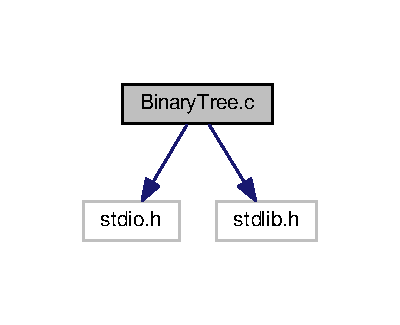
\includegraphics[width=192pt]{BinaryTree_8c__incl}
\end{center}
\end{figure}
\subsection*{Classes}
\begin{DoxyCompactItemize}
\item 
struct \hyperlink{structgrafo}{grafo}
\end{DoxyCompactItemize}
\subsection*{Typedefs}
\begin{DoxyCompactItemize}
\item 
typedef struct \hyperlink{structgrafo}{grafo} \hyperlink{BinaryTree_8c_acf45bb9708cd063385a2b5a86675e560}{G\+R\+A\+FO}
\end{DoxyCompactItemize}
\subsection*{Functions}
\begin{DoxyCompactItemize}
\item 
struct \hyperlink{structgrafo}{grafo} $\ast$ \hyperlink{BinaryTree_8c_a48a10a9c61592d8e677efe924630dd91}{cria} ()
\item 
struct \hyperlink{structgrafo}{grafo} $\ast$ \hyperlink{BinaryTree_8c_a8e3be2dca8e187f4d2057cd6a9a42f5c}{insere} (\hyperlink{BinaryTree_8c_acf45bb9708cd063385a2b5a86675e560}{G\+R\+A\+FO} $\ast$G, int elem)
\item 
void \hyperlink{BinaryTree_8c_a09bff38a7fb2a4db0a4f9a679fede3eb}{preO} (\hyperlink{BinaryTree_8c_acf45bb9708cd063385a2b5a86675e560}{G\+R\+A\+FO} $\ast$G)
\item 
void \hyperlink{BinaryTree_8c_ae3d4992ae457ee9ec2c89b59a95d3444}{posO} (\hyperlink{BinaryTree_8c_acf45bb9708cd063385a2b5a86675e560}{G\+R\+A\+FO} $\ast$G)
\item 
void \hyperlink{BinaryTree_8c_aaf490eb1d7cdd1daaed9589fb8a65f48}{intO} (\hyperlink{BinaryTree_8c_acf45bb9708cd063385a2b5a86675e560}{G\+R\+A\+FO} $\ast$G)
\item 
int \hyperlink{BinaryTree_8c_ae66f6b31b5ad750f1fe042a706a4e3d4}{main} ()
\end{DoxyCompactItemize}


\subsection{Typedef Documentation}
\index{Binary\+Tree.\+c@{Binary\+Tree.\+c}!G\+R\+A\+FO@{G\+R\+A\+FO}}
\index{G\+R\+A\+FO@{G\+R\+A\+FO}!Binary\+Tree.\+c@{Binary\+Tree.\+c}}
\subsubsection[{\texorpdfstring{G\+R\+A\+FO}{GRAFO}}]{\setlength{\rightskip}{0pt plus 5cm}typedef struct {\bf grafo} {\bf G\+R\+A\+FO}}\hypertarget{BinaryTree_8c_acf45bb9708cd063385a2b5a86675e560}{}\label{BinaryTree_8c_acf45bb9708cd063385a2b5a86675e560}


\subsection{Function Documentation}
\index{Binary\+Tree.\+c@{Binary\+Tree.\+c}!cria@{cria}}
\index{cria@{cria}!Binary\+Tree.\+c@{Binary\+Tree.\+c}}
\subsubsection[{\texorpdfstring{cria()}{cria()}}]{\setlength{\rightskip}{0pt plus 5cm}struct {\bf grafo}$\ast$ cria (
\begin{DoxyParamCaption}
{}
\end{DoxyParamCaption}
)}\hypertarget{BinaryTree_8c_a48a10a9c61592d8e677efe924630dd91}{}\label{BinaryTree_8c_a48a10a9c61592d8e677efe924630dd91}

\begin{DoxyCode}
13 \{
14     \textcolor{keywordflow}{return} NULL;
15 \};
\end{DoxyCode}
\index{Binary\+Tree.\+c@{Binary\+Tree.\+c}!insere@{insere}}
\index{insere@{insere}!Binary\+Tree.\+c@{Binary\+Tree.\+c}}
\subsubsection[{\texorpdfstring{insere(\+G\+R\+A\+F\+O $\ast$\+G, int elem)}{insere(GRAFO *G, int elem)}}]{\setlength{\rightskip}{0pt plus 5cm}struct {\bf grafo}$\ast$ insere (
\begin{DoxyParamCaption}
\item[{{\bf G\+R\+A\+FO} $\ast$}]{G, }
\item[{int}]{elem}
\end{DoxyParamCaption}
)}\hypertarget{BinaryTree_8c_a8e3be2dca8e187f4d2057cd6a9a42f5c}{}\label{BinaryTree_8c_a8e3be2dca8e187f4d2057cd6a9a42f5c}

\begin{DoxyCode}
17                                         \{
18 
19     \hyperlink{structgrafo}{GRAFO} *gr = (\hyperlink{structgrafo}{GRAFO}*)malloc(\textcolor{keyword}{sizeof}(\textcolor{keyword}{struct} \hyperlink{structgrafo}{grafo})),*aux,*ant;
20     aux = G;
21     \textcolor{keywordflow}{if}(!gr)\textcolor{keywordflow}{return} G;
22     gr->\hyperlink{structgrafo_a9f3a642f8e0a5350f2a4896d3db685ee}{i} = elem;
23     gr->\hyperlink{structgrafo_acefee7ad605f204f8b1bd063adfac34c}{dir} = NULL;
24     gr->\hyperlink{structgrafo_a258a14d55dea22c0507102319671226f}{esq} = NULL;
25 
26     \textcolor{keywordflow}{if}(!G)
27         \textcolor{keywordflow}{return} gr;
28 
29     \textcolor{keywordflow}{while}(1)
30     \{
31 
32         \textcolor{keywordflow}{if}(aux->i<elem)
33         \{
34             \textcolor{keywordflow}{if}(aux->dir!=NULL)\{
35                 aux = aux->\hyperlink{structgrafo_acefee7ad605f204f8b1bd063adfac34c}{dir};
36             \}
37             \textcolor{keywordflow}{else} \textcolor{keywordflow}{if}(aux->dir == NULL)\{
38                 aux->\hyperlink{structgrafo_acefee7ad605f204f8b1bd063adfac34c}{dir} = gr;
39                 \textcolor{keywordflow}{return} G;
40             \}
41         \}
42         \textcolor{keywordflow}{else} \textcolor{keywordflow}{if}(aux->i>elem)
43         \{
44             \textcolor{keywordflow}{if}(aux->esq!=NULL)\{
45                 aux = aux->\hyperlink{structgrafo_a258a14d55dea22c0507102319671226f}{esq};
46             \}
47             \textcolor{keywordflow}{else} \textcolor{keywordflow}{if}(aux->esq == NULL)\{
48                 aux->\hyperlink{structgrafo_a258a14d55dea22c0507102319671226f}{esq} = gr;
49                 \textcolor{keywordflow}{return} G;
50             \}
51         \}
52     \}
53 \};
\end{DoxyCode}
\index{Binary\+Tree.\+c@{Binary\+Tree.\+c}!intO@{intO}}
\index{intO@{intO}!Binary\+Tree.\+c@{Binary\+Tree.\+c}}
\subsubsection[{\texorpdfstring{int\+O(\+G\+R\+A\+F\+O $\ast$\+G)}{intO(GRAFO *G)}}]{\setlength{\rightskip}{0pt plus 5cm}void intO (
\begin{DoxyParamCaption}
\item[{{\bf G\+R\+A\+FO} $\ast$}]{G}
\end{DoxyParamCaption}
)}\hypertarget{BinaryTree_8c_aaf490eb1d7cdd1daaed9589fb8a65f48}{}\label{BinaryTree_8c_aaf490eb1d7cdd1daaed9589fb8a65f48}

\begin{DoxyCode}
76 \{
77     \textcolor{keywordflow}{if}(G)
78     \{
79         \hyperlink{BinaryTree_8c_aaf490eb1d7cdd1daaed9589fb8a65f48}{intO}(G->\hyperlink{structgrafo_a258a14d55dea22c0507102319671226f}{esq});
80         printf(\textcolor{stringliteral}{" %d"},G->\hyperlink{structgrafo_a9f3a642f8e0a5350f2a4896d3db685ee}{i});
81         \hyperlink{BinaryTree_8c_aaf490eb1d7cdd1daaed9589fb8a65f48}{intO}(G->\hyperlink{structgrafo_acefee7ad605f204f8b1bd063adfac34c}{dir});
82     \}
83 \}
\end{DoxyCode}
\index{Binary\+Tree.\+c@{Binary\+Tree.\+c}!main@{main}}
\index{main@{main}!Binary\+Tree.\+c@{Binary\+Tree.\+c}}
\subsubsection[{\texorpdfstring{main()}{main()}}]{\setlength{\rightskip}{0pt plus 5cm}int main (
\begin{DoxyParamCaption}
{}
\end{DoxyParamCaption}
)}\hypertarget{BinaryTree_8c_ae66f6b31b5ad750f1fe042a706a4e3d4}{}\label{BinaryTree_8c_ae66f6b31b5ad750f1fe042a706a4e3d4}

\begin{DoxyCode}
85           \{
86     \textcolor{keywordtype}{int} a,b,c,d=1;
87     \hyperlink{structgrafo}{GRAFO} *g = \hyperlink{BinaryTree_8c_a48a10a9c61592d8e677efe924630dd91}{cria}();
88     scanf(\textcolor{stringliteral}{"%d"},&a);
89     \textcolor{keywordflow}{while}(a--)
90     \{
91         scanf(\textcolor{stringliteral}{"%d"},&b);
92         \textcolor{keywordflow}{while}(b--)
93         \{
94             scanf(\textcolor{stringliteral}{"%d"},&c);
95             g = \hyperlink{BinaryTree_8c_a8e3be2dca8e187f4d2057cd6a9a42f5c}{insere}(g,c);
96         \}
97         printf(\textcolor{stringliteral}{"Case %d:\(\backslash\)n"},d++);
98         printf(\textcolor{stringliteral}{"Pre.:"});
99         \hyperlink{BinaryTree_8c_a09bff38a7fb2a4db0a4f9a679fede3eb}{preO}(g);
100         printf(\textcolor{stringliteral}{"\(\backslash\)nIn..:"});
101         \hyperlink{BinaryTree_8c_aaf490eb1d7cdd1daaed9589fb8a65f48}{intO}(g);
102         printf(\textcolor{stringliteral}{"\(\backslash\)nPost:"});
103         \hyperlink{BinaryTree_8c_ae3d4992ae457ee9ec2c89b59a95d3444}{posO}(g);
104         printf(\textcolor{stringliteral}{"\(\backslash\)n\(\backslash\)n"});
105         g = \hyperlink{BinaryTree_8c_a48a10a9c61592d8e677efe924630dd91}{cria}();
106     \}
107 \}\end{DoxyCode}


Here is the call graph for this function\+:
\nopagebreak
\begin{figure}[H]
\begin{center}
\leavevmode
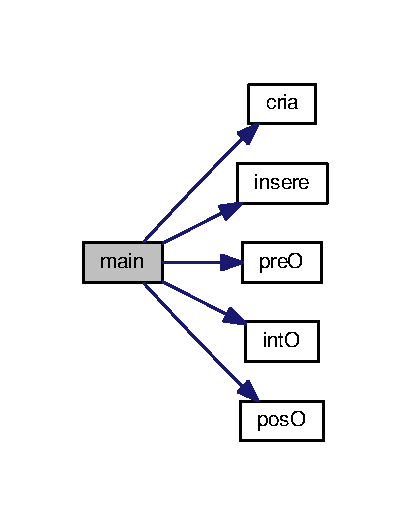
\includegraphics[width=197pt]{BinaryTree_8c_ae66f6b31b5ad750f1fe042a706a4e3d4_cgraph}
\end{center}
\end{figure}


\index{Binary\+Tree.\+c@{Binary\+Tree.\+c}!posO@{posO}}
\index{posO@{posO}!Binary\+Tree.\+c@{Binary\+Tree.\+c}}
\subsubsection[{\texorpdfstring{pos\+O(\+G\+R\+A\+F\+O $\ast$\+G)}{posO(GRAFO *G)}}]{\setlength{\rightskip}{0pt plus 5cm}void posO (
\begin{DoxyParamCaption}
\item[{{\bf G\+R\+A\+FO} $\ast$}]{G}
\end{DoxyParamCaption}
)}\hypertarget{BinaryTree_8c_ae3d4992ae457ee9ec2c89b59a95d3444}{}\label{BinaryTree_8c_ae3d4992ae457ee9ec2c89b59a95d3444}

\begin{DoxyCode}
66 \{
67     \textcolor{keywordflow}{if}(G)
68     \{
69         \hyperlink{BinaryTree_8c_ae3d4992ae457ee9ec2c89b59a95d3444}{posO}(G->\hyperlink{structgrafo_a258a14d55dea22c0507102319671226f}{esq});
70         \hyperlink{BinaryTree_8c_ae3d4992ae457ee9ec2c89b59a95d3444}{posO}(G->\hyperlink{structgrafo_acefee7ad605f204f8b1bd063adfac34c}{dir});
71         printf(\textcolor{stringliteral}{" %d"},G->\hyperlink{structgrafo_a9f3a642f8e0a5350f2a4896d3db685ee}{i});
72     \}
73 \}
\end{DoxyCode}
\index{Binary\+Tree.\+c@{Binary\+Tree.\+c}!preO@{preO}}
\index{preO@{preO}!Binary\+Tree.\+c@{Binary\+Tree.\+c}}
\subsubsection[{\texorpdfstring{pre\+O(\+G\+R\+A\+F\+O $\ast$\+G)}{preO(GRAFO *G)}}]{\setlength{\rightskip}{0pt plus 5cm}void preO (
\begin{DoxyParamCaption}
\item[{{\bf G\+R\+A\+FO} $\ast$}]{G}
\end{DoxyParamCaption}
)}\hypertarget{BinaryTree_8c_a09bff38a7fb2a4db0a4f9a679fede3eb}{}\label{BinaryTree_8c_a09bff38a7fb2a4db0a4f9a679fede3eb}

\begin{DoxyCode}
56 \{
57     \textcolor{keywordflow}{if}(G)
58     \{
59         printf(\textcolor{stringliteral}{" %d"},G->\hyperlink{structgrafo_a9f3a642f8e0a5350f2a4896d3db685ee}{i});
60         \hyperlink{BinaryTree_8c_a09bff38a7fb2a4db0a4f9a679fede3eb}{preO}(G->\hyperlink{structgrafo_a258a14d55dea22c0507102319671226f}{esq});
61         \hyperlink{BinaryTree_8c_a09bff38a7fb2a4db0a4f9a679fede3eb}{preO}(G->\hyperlink{structgrafo_acefee7ad605f204f8b1bd063adfac34c}{dir});
62     \}
63 \}
\end{DoxyCode}

%--- End generated contents ---

% Index
\backmatter
\newpage
\phantomsection
\clearemptydoublepage
\addcontentsline{toc}{chapter}{Index}
\printindex

\end{document}
